\chapter{Reconnaissance des chiffres manuscrits}

\section{La base de données MNIST}

\subsection{Présentation de MNIST}
La base de données MNIST (ou Mixed National Institute of Standards and Technology) est un regroupement de 70 000 chiffres manuscrits. 60 000 d'entre eux servent à l'apprentissage et les 10 000 autres permettent de tester le réseau de neurones après l'apprentissage. Ce sont des images normalisées en noir et blanc, de 28 pixels de côté chacun codé sur un octet. Nous nous appuierons sur cette base de données pour faire apprendre à notre réseau de neurones la reconnaissance de chiffres.

\begin{figure}[h]
\begin{center}
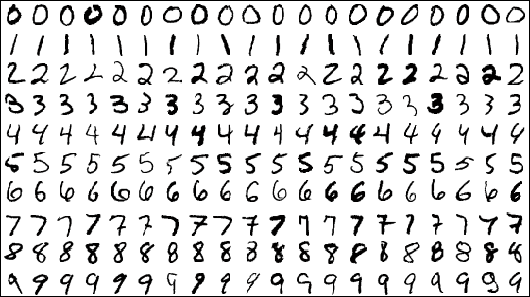
\includegraphics[width=0.6\textwidth]{images/mnistExamples.png}\caption{Exemples d'images tirées de la base de données MNIST. Chaque chiffre fait 28 pixels de côté}
\end{center}
\end{figure}

\subsection{Extraction de MNIST} 
Les données sont dans le format idx1 et idx3 tel que : \\ \\
\begin{tabular}{|c | c | c | c|}
\hline
\textbf{offset} & \textbf{type} & \textbf{valeur} & \textbf{description} \\
\hline
0000 & 32 bit integer & 0x00000803(2051) & magic number\\
0004 & 32 bit integer & 60000 & number of items\\
0008 & 32 bit integer & 28 & number of rows \\
0012 & 32 bit integer & 28 & number of columns \\
0016 & unsigned byte & ?? & pixel\\
0017 & unsigned byte & ?? & pixel\\
... & ... & ... & ... \\
xxxx  &  unsigned byte & ?? & pixel\\
\hline
\end{tabular} \\ \\
On peut distinguer :
\begin{itemize}
  \item Le \textit{magic number} qui permet d'identifier le format de la base de données
  \item Les \textit{number of items, number of rows, number of colums} donne des informations sur les données, ce qui nous permettra d'extraire les images
  \item Les \textit{pixels} qui sont les octets en niveau de gris des images
\end{itemize} 
L'extraction se fait donc en lisant successivement les octets et en les stockant dans des \textit{vector<Eigen:Matrix>} grâce aux données récupérées. En faisant de même avec les labels dont le format est très sensiblement le même, on obtient une liste de vecteur colonne d'\textit{Eigen::Matrix} de taille 784 (28*28) ainsi que leur label sur un autre \textit{Eigen::Matrix}. On fait de même avec les échantillons de test et on est fin prêt pour l'apprentissage.

\section{Apprentissage de la base de données}
\subsection{Paramétrage du réseau de neurones}
Bien que le format de l'entrée soit le même (vecteur colonne si ce n'est la taille qui change), un réseau à 3 ou 4 neurones ne suffit pas. Il a fallu adapter de façon empirique les différents paramètres. On peut jouer sur :
\begin{itemize}
  \item Le nombre de neurones
  \item Le nombre de couches
  \item Le pas d'apprentissage
  \item Les fonctions d'activations par couches
  \item Le nombre d'apprentissages
\end{itemize}
\subsubsection{Le nombre de couches et de neurones}

\subsubsection{Le pas d'apprentissage}

\subsubsection{Les fonctions d'activations par couches}

\subsubsection{Le nombre d'apprentissages}

\subsection{Résultat}

